\documentclass[tikz,border=10pt]{standalone}
\usepackage{tikz}
\usetikzlibrary{shapes.geometric, arrows.meta, positioning, shadows, backgrounds, fit, calc}
\usepackage{fontawesome5}

\definecolor{nexusIndigo}{RGB}{99,102,241}
\definecolor{nexusPurple}{RGB}{139,92,246}
\definecolor{nexusPink}{RGB}{236,72,153}
\definecolor{nexusGray}{RGB}{107,114,128}
\definecolor{nexusLightGray}{RGB}{243,244,246}
\definecolor{nexusSuccess}{RGB}{34,197,94}
\definecolor{nexusWarning}{RGB}{251,146,60}

% Define styles
\tikzstyle{stage} = [rectangle, rounded corners, minimum width=3cm, minimum height=1cm, text centered, draw=black, fill=nexusIndigo!20, drop shadow, font=\bfseries]
\tikzstyle{process} = [rectangle, rounded corners, minimum width=2.5cm, minimum height=0.8cm, text centered, draw=nexusPurple, fill=nexusPurple!10, font=\small]
\tikzstyle{data} = [cylinder, shape border rotate=90, aspect=0.25, minimum width=2cm, minimum height=1cm, draw=nexusSuccess, fill=nexusSuccess!10, font=\small]
\tikzstyle{api} = [ellipse, minimum width=2cm, minimum height=0.8cm, draw=nexusPink, fill=nexusPink!10, font=\small]
\tikzstyle{decision} = [diamond, aspect=2, minimum width=2cm, minimum height=1cm, draw=nexusWarning, fill=nexusWarning!10, font=\small]
\tikzstyle{arrow} = [thick,-{Stealth[length=3mm]},>=stealth]
\tikzstyle{doublearrow} = [thick,{Stealth[length=3mm]}-{Stealth[length=3mm]},>=stealth]
\tikzstyle{label} = [font=\tiny, text=nexusGray]

\begin{document}

\begin{tikzpicture}[node distance=1.5cm, scale=0.85, every node/.style={scale=0.85}]

% ========== TITLE ==========
\node[font=\Huge\bfseries, text=nexusIndigo] at (8,17) {NEXUS - AI-Powered Career Analytics Platform};
\node[font=\large, text=nexusGray] at (8,16.2) {Complete Data Pipeline \& Architecture};

% ========== STAGE 1: DATA ACQUISITION ==========
\node[stage] (stage1) at (0,14) {STAGE 1: DATA ACQUISITION};

\node[api] (kaggle) [below=of stage1] {\faIcon{kaggle} Kaggle API};
\node[data] (rawdata) [below=of kaggle] {Raw Dataset\\jobs\_in\_data.csv\\5000+ records};

\draw[arrow] (stage1) -- (kaggle);
\draw[arrow] (kaggle) -- node[label, right] {Download} (rawdata);

% Dataset details
\node[process, align=left, minimum width=3.5cm] (dataset-info) [right=1.5cm of rawdata] {
    \textbf{Dataset Fields:}\\
    • Job Title\\
    • Company\\
    • Location\\
    • Work Type\\
    • Experience Level\\
    • Skills Required\\
    • LinkedIn URL
};

% ========== STAGE 2: DATA CLEANING ==========
\node[stage] (stage2) at (0,8.5) {STAGE 2: DATA CLEANING};

\node[process] (remove-null) [below=0.8cm of stage2] {Remove NULL\\Values};
\node[process] (remove-dup) [below=of remove-null] {Remove\\Duplicates};
\node[process] (standardize) [below=of remove-dup] {Standardize\\Formats};
\node[data] (cleandata) [below=of standardize] {Clean Dataset\\4800+ records};

\draw[arrow] (rawdata) -- (stage2);
\draw[arrow] (stage2) -- (remove-null);
\draw[arrow] (remove-null) -- (remove-dup);
\draw[arrow] (remove-dup) -- (standardize);
\draw[arrow] (standardize) -- (cleandata);

% Cleaning details
\node[process, align=left, minimum width=3cm] (clean-info) [right=1.5cm of remove-dup] {
    \textbf{Cleaning Steps:}\\
    • Drop rows with NaN\\
    • Remove exact duplicates\\
    • Normalize text case\\
    • Trim whitespaces\\
    • Validate data types
};

% ========== STAGE 3: PREPROCESSING ==========
\node[stage] (stage3) at (8,8.5) {STAGE 3: PREPROCESSING};

\node[process] (tokenize) [below=0.8cm of stage3] {Tokenize\\Skills};
\node[process] (vectorize) [below=of tokenize] {TF-IDF\\Vectorization};
\node[process] (encode) [below=of vectorize] {Label\\Encoding};
\node[data] (features) [below=of encode] {Feature Matrix\\X, y};

\draw[arrow] (cleandata) -- (stage3);
\draw[arrow] (stage3) -- (tokenize);
\draw[arrow] (tokenize) -- (vectorize);
\draw[arrow] (vectorize) -- (encode);
\draw[arrow] (encode) -- (features);

% Preprocessing details
\node[process, align=left, minimum width=3.5cm] (preprocess-info) [right=1.5cm of vectorize] {
    \textbf{Feature Engineering:}\\
    • Skills → TF-IDF vectors\\
    • Experience → Numeric\\
    • Location → Encoded\\
    • Work Type → Encoded\\
    • Job Title → Target
};

% ========== STAGE 4: MODEL TRAINING ==========
\node[stage] (stage4) at (8,2.5) {STAGE 4: MODEL TRAINING};

\node[process] (split) [below=0.8cm of stage4] {Train/Test\\Split (80/20)};
\node[process] (knn) [below left=0.8cm and -0.5cm of split] {K-Nearest\\Neighbors\\(k=5)};
\node[process] (lwr) [below right=0.8cm and -0.5cm of split] {Locally Weighted\\Regression\\(sklearn)};
\node[data] (model) [below=1.5cm of split] {Trained Models\\KNN + LWR};

\draw[arrow] (features) -- (stage4);
\draw[arrow] (stage4) -- (split);
\draw[arrow] (split) -- (knn);
\draw[arrow] (split) -- (lwr);
\draw[arrow] (knn) -- (model);
\draw[arrow] (lwr) -- (model);

% Model details
\node[process, align=left, minimum width=3.5cm] (model-info) [right=1.5cm of split] {
    \textbf{Training Details:}\\
    • Algorithm: KNN\\
    • Distance: Weighted\\
    • Features: 100+ dims\\
    • Accuracy: 85\%+\\
    • Framework: scikit-learn
};

% ========== STAGE 5: BACKEND API ==========
\node[stage] (stage5) at (16,8.5) {STAGE 5: BACKEND API};

\node[api] (fastapi) [below=0.8cm of stage5] {\faIcon{python} FastAPI\\uvicorn};
\node[process] (predict-endpoint) [below left=0.8cm and 0.5cm of fastapi] {POST\\/api/predict-jobs};
\node[process] (cors) [below right=0.8cm and 0.5cm of fastapi] {CORS\\Middleware};
\node[data] (backend-db) [below=1.5cm of fastapi] {Jobs Database\\PostgreSQL/JSON};

\draw[arrow] (model) -- (stage5);
\draw[arrow] (stage5) -- (fastapi);
\draw[arrow] (fastapi) -- (predict-endpoint);
\draw[arrow] (fastapi) -- (cors);
\draw[arrow] (backend-db) -- (fastapi);

% Backend details
\node[process, align=left, minimum width=3.5cm] (backend-info) [right=1.5cm of fastapi] {
    \textbf{Backend Stack:}\\
    • FastAPI (Python)\\
    • Port: 8000\\
    • Auto docs: /docs\\
    • CORS enabled\\
    • Hot reload dev mode
};

% ========== STAGE 6: CV PARSING ==========
\node[stage] (stage6) at (16,2.5) {STAGE 6: CV PARSING};

\node[api] (pdfjs) [below=0.8cm of stage6] {\faIcon{file-pdf} PDF.js\\Library};
\node[process] (extract-text) [below left=0.8cm and 0cm of pdfjs] {Extract\\Text};
\node[process] (parse-sections) [below right=0.8cm and 0cm of pdfjs] {Parse\\Sections};
\node[process] (extract-skills) [below=1.5cm of pdfjs] {Extract Skills,\\Education,\\Projects};
\node[data] (cv-data) [below=of extract-skills] {Structured\\CV Data};

\draw[doublearrow] (backend-db) -- node[label, right] {Query jobs} (stage6);
\draw[arrow] (stage6) -- (pdfjs);
\draw[arrow] (pdfjs) -- (extract-text);
\draw[arrow] (pdfjs) -- (parse-sections);
\draw[arrow] (extract-text) -- (extract-skills);
\draw[arrow] (parse-sections) -- (extract-skills);
\draw[arrow] (extract-skills) -- (cv-data);

% CV Parsing details
\node[process, align=left, minimum width=3.5cm] (cv-info) [right=1.5cm of extract-skills] {
    \textbf{CV Parsing:}\\
    • PDF.js v2.x\\
    • Regex patterns\\
    • NLP techniques\\
    • Field detection\\
    • Skill extraction
};

% ========== STAGE 7: FRONTEND ==========
\node[stage] (stage7) at (16,-3.5) {STAGE 7: FRONTEND};

\node[api] (react) [below=0.8cm of stage7] {\faIcon{react} React 18\\+ Vite};
\node[process] (upload) [below left=0.8cm and 1cm of react] {CV Upload\\Component};
\node[process] (dashboard) [below=1.2cm of react] {Results\\Dashboard};
\node[process] (coverletter) [below right=0.8cm and 1cm of react] {Cover Letter\\Generator};

\draw[arrow] (cv-data) -- (stage7);
\draw[arrow] (stage7) -- (react);
\draw[arrow] (react) -- (upload);
\draw[arrow] (react) -- (dashboard);
\draw[arrow] (react) -- (coverletter);

% Frontend details
\node[process, align=left, minimum width=3.5cm] (frontend-info) [right=1.5cm of react] {
    \textbf{Frontend Stack:}\\
    • React 18\\
    • Vite bundler\\
    • Tailwind CSS\\
    • Framer Motion\\
    • Lucide Icons\\
    • Port: 5173-5175
};

% ========== STAGE 8: EXTERNAL APIS ==========
\node[stage] (stage8) at (8,-3.5) {STAGE 8: EXTERNAL APIs};

\node[api] (clearbit) [below left=0.8cm and 0cm of stage8] {\faIcon{image} Clearbit\\Logo API};
\node[api] (linkedin) [below right=0.8cm and 0cm of stage8] {\faIcon{linkedin} LinkedIn\\Integration};
\node[process] (jspdf) [below=1.5cm of stage8] {jsPDF\\PDF Generation};

\draw[doublearrow] (coverletter) -- (stage8);
\draw[arrow] (stage8) -- (clearbit);
\draw[arrow] (stage8) -- (linkedin);
\draw[arrow] (stage8) -- (jspdf);

% External APIs details
\node[process, align=left, minimum width=3.5cm] (api-info) [left=1.5cm of stage8] {
    \textbf{Third-party APIs:}\\
    • Clearbit: Company logos\\
    • LinkedIn: Job links\\
    • jsPDF: Cover letters\\
    • Font Awesome: Icons
};

% ========== STAGE 9: USER INTERFACE ==========
\node[stage] (stage9) at (8,-8) {STAGE 9: USER INTERFACE};

\node[process] (home) [below left=0.8cm and 1.5cm of stage9] {Home Page\\Landing};
\node[process] (results) [below=1.2cm of stage9] {Job Predictions\\Display};
\node[process] (pdf-gen) [below right=0.8cm and 1.5cm of stage9] {PDF Download\\Feature};

\draw[arrow] (upload) -- (stage9);
\draw[arrow] (dashboard) -- (stage9);
\draw[arrow] (coverletter) -- (stage9);
\draw[arrow] (stage9) -- (home);
\draw[arrow] (stage9) -- (results);
\draw[arrow] (stage9) -- (pdf-gen);

% UI details
\node[process, align=left, minimum width=3.5cm] (ui-info) [right=1.5cm of results] {
    \textbf{UI Features:}\\
    • Responsive design\\
    • Dark/Light themes\\
    • Animations\\
    • File drag \& drop\\
    • Real-time validation
};

% ========== DATA FLOW CONNECTIONS ==========
\draw[arrow, nexusPurple, very thick] (predict-endpoint) to[out=270,in=90] node[label, left, align=center] {POST CV data\\Get predictions} (dashboard);
\draw[arrow, nexusPink, very thick] (clearbit) to[out=180,in=0] node[label, below] {Fetch logos} (results);
\draw[arrow, nexusSuccess, very thick] (jspdf) -- node[label, right] {Generate PDF} (pdf-gen);

% ========== LEGEND ==========
\node[font=\bfseries, text=nexusIndigo] at (0,-9.5) {LEGEND:};
\node[stage, minimum width=2cm] at (2,-9.5) {Stage};
\node[process, minimum width=2cm] at (5,-9.5) {Process};
\node[data, minimum width=2cm] at (8,-9.5) {Data Store};
\node[api, minimum width=2cm] at (11,-9.5) {API/Library};

% ========== TECH STACK BOX ==========
\node[draw=nexusIndigo, fill=nexusLightGray, rounded corners, align=left, minimum width=14cm, minimum height=2.5cm] at (8,-12) {
    \textbf{\Large Technology Stack:}\\[0.3cm]
    \textbf{Frontend:} React 18, Vite, Tailwind CSS, Framer Motion, Lucide Icons, React Router\\
    \textbf{Backend:} Python 3.10+, FastAPI, Uvicorn, Pydantic, CORS Middleware\\
    \textbf{ML/AI:} scikit-learn, pandas, numpy, K-Nearest Neighbors, Locally Weighted Regression\\
    \textbf{Data Processing:} PDF.js, TF-IDF Vectorization, Regular Expressions, NLP\\
    \textbf{PDF Generation:} jsPDF v2.5.1\\
    \textbf{External APIs:} Clearbit Logo API, LinkedIn\\
    \textbf{Development:} Git, VS Code, npm, pip, Hot Module Replacement
};

% ========== FOOTER ==========
\node[font=\small, text=nexusGray] at (8,-14) {© 2025 NEXUS - AI-Powered Career Analytics Platform | Complete Pipeline Documentation};

\end{tikzpicture}

\end{document}
